\documentclass{sig-alternate}
\usepackage[T1]{fontenc}
\usepackage{array}
\usepackage{verbatim}
\usepackage{booktabs}
\usepackage{fancyvrb}
\usepackage{url}
\usepackage[english]{babel}
\usepackage{listings}

\makeatletter
\makeatother

\begin{document}

%\author{BLINDED FOR SUBMISSION}

\title{Give 'em less rope: Open Source Evidence of Java Sandbox Perversions}

\numberofauthors{1} 
\author{\alignauthor Zack Coker, Michael Maass, Tianyuan Ding, Claire Le Goues, and Joshua Sunshine \\
\affaddr{Carnegie Mellon University} \\
\email{\{zfc,mmass\}@cs.cmu.edu, tding@cmu.edu, \{clegoues,sunshine\}@cs.cmu.edu}
} 

\maketitle
%JSS: This is to force page numbers.
\thispagestyle{plain} 
\pagestyle{plain}
\begin{abstract}
The ubiquitously-installed Java Runtime Environment (JRE) executes
untrusted code inside a sandbox to protect the host machine from potential
malicious behavior. However, dozens of recent exploits have successfully
escaped the sandbox, thereby enabling attackers to infect countless
Java hosts. It is essential to distinguish patterns of malicious use
from patterns of benign use to proactively prevent future exploits.
We therefore performed an empirical study of benign open-source Java
applications and compared their use of the sandbox to the usage present
in recent exploits. We found that benign applications with secured
sandboxes do not modify the security manager, the security policy
enforcement mechanism, after it is first set and do not attempt to
directly use privileged classes. Exploits routinely do both. We derive two rules from these results to prevent (1) security manager modifications and (2) privilege escalation. We evaluated their protection merits in a case study using runtime monitors to enforce the rules during the execution of exploits and benign applications. The rules stop all ten Metasploit Java 7 exploits without breaking backwards compatibility with benign applications. These practical rules should be enforced in the JRE to fortify the Java sandbox.
\end{abstract}

\section{Introduction}

The Java Runtime Environment (JRE) is widely installed on user endpoints,
where it executes external code in the form of applets and Java Web Start (JWS) \cite{_java_web_start} applications \cite{gong1997going,gong2003inside}.
These facts, combined with the hundreds of recently discovered vulnerabilities
in Java, including zero-day vulnerabilities (e.g. CVE-2013-0422),
have made Java a popular exploit vector (see Figure \ref{fig:most-targeted-applications}).
Attackers typically lure users to websites containing hidden malicious
applets. Once the user visits the website, the exploit triggers a
series of events that ends with the delivery of malware, all while
the user is left unaware. This kind of attack is commonly referred
to as a ``drive-by download.''

Java includes a mechanism to safely execute untrusted code and isolate
components from one another in a sandbox, such that both the application
and the host machine are protected from malicious behavior. However,
the exploits cited above show that there is substantial room to improve
the containment of code within the sandbox. Previous investigations
of Java exploits have shown Java malware commonly alters the sandbox's
settings \cite{garber_2012}. Typically, exploits disable the security
manager, the component of the sandbox responsible for enforcing the
security policy \cite{fireeye_2013,svoboda_anatomy_blog_2013,security_explorations_2012,blackhat_2012}.
We hypothesize that, when compared to the exploits, benign applications
interact with the security manager differently. If true, this difference
can be exploited to prevent future attacks.

\begin{figure}
\begin{centering}
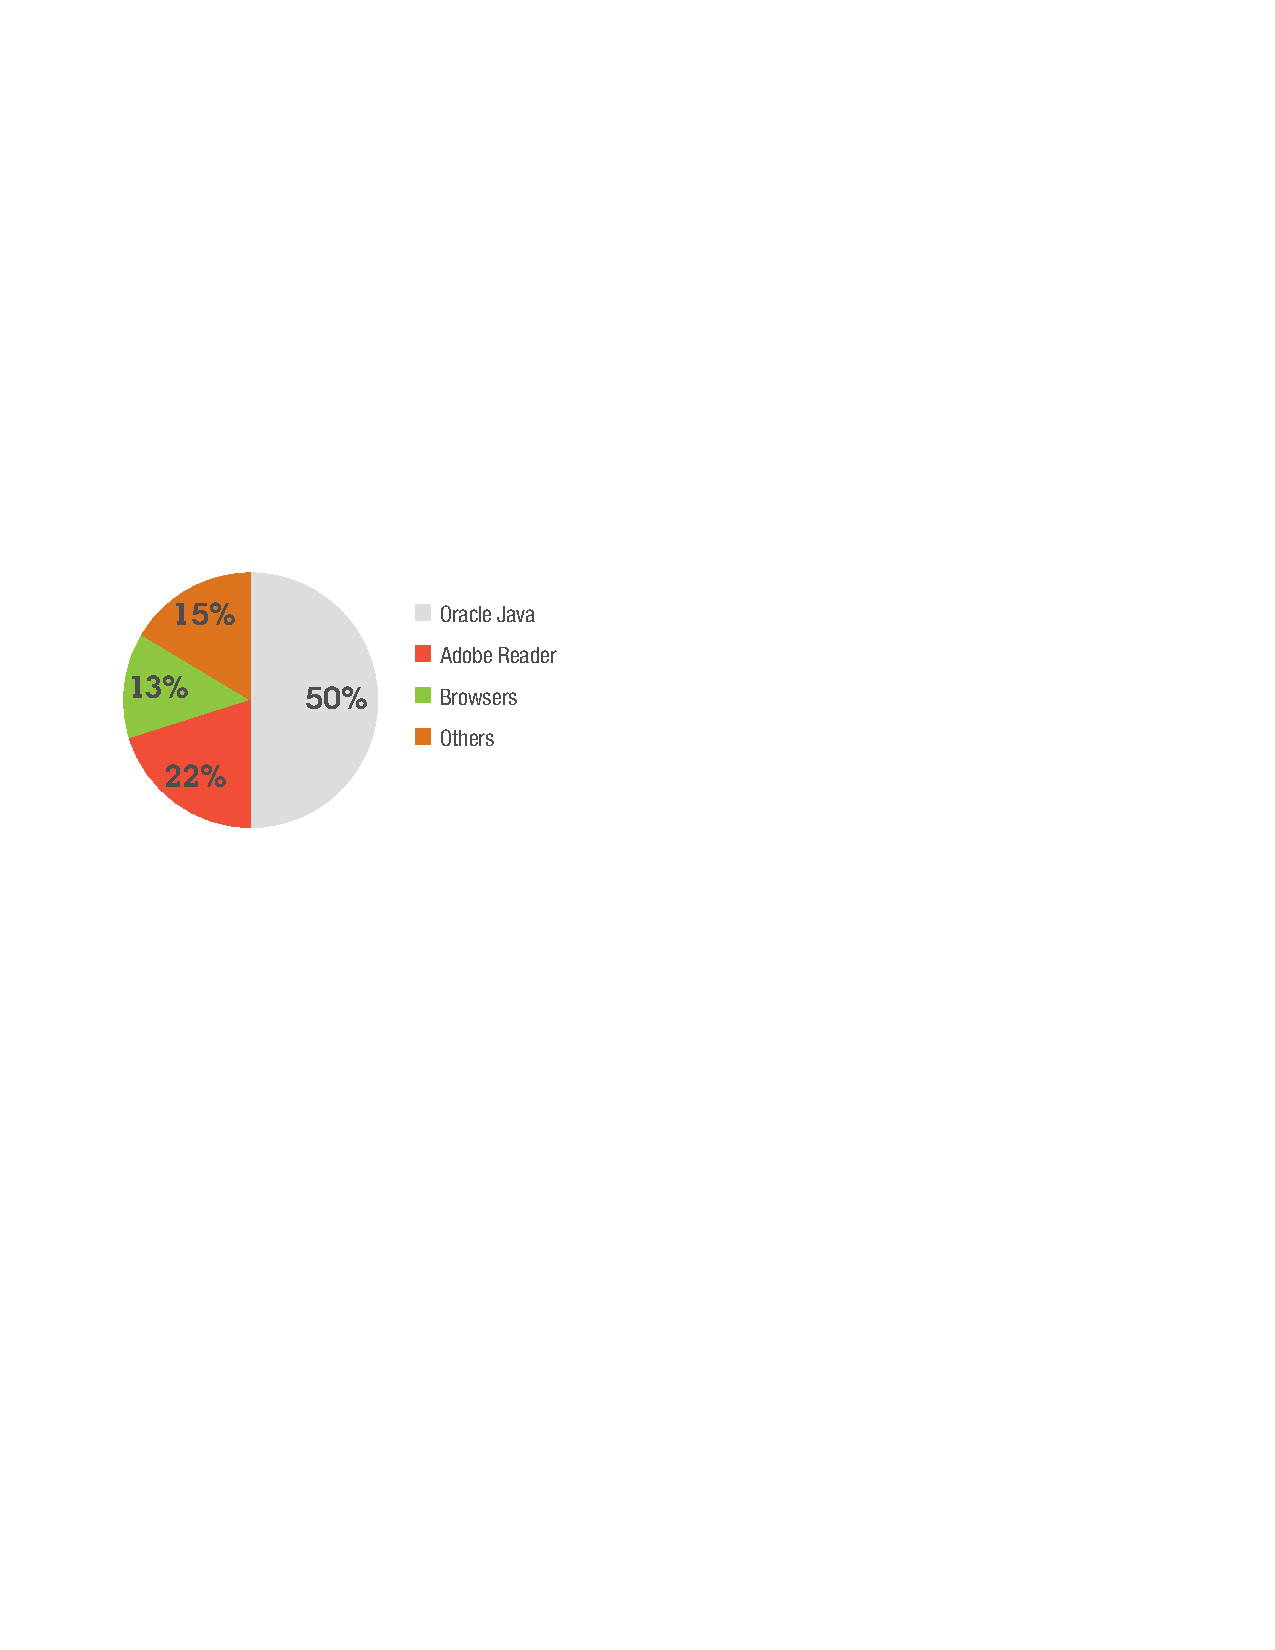
\includegraphics[width=2in]{most_targeted_apps_ibm_xforce}
\par\end{centering}

\caption{Pie chart showing the most
targeted applications on enterprise workstations, according to to
a Dec. 2013 survey of Trusteer customers \cite{xforceQ12013}. Java
represented half of all attack-attempts in their sample.}
\label{fig:most-targeted-applications}
\end{figure}

To validate this insight, we conducted an empirical study of benign
open source Java applications. Our empirical study was designed to
answer the following research question: How do benign applications
modify the security manager? To answer this question, we identified
Java projects in the Qualitas Corpus \cite{QualitasCorpus:APSEC:2010}
and the GitHub repository that make use of the security manager. We
analyzed the resulting 46 projects using a custom FindBugs \cite{hovemeyer_finding_2004}
plugin to isolate code involved in the initialization or modification
of the security manager. We then manually characterized the security
manager usage in each of the isolated code snippets. Finally, we used
a Java Virtual Machine Tool Interface (JVMTI) agent to confirm that
our characterizations were accurate at run time. 

We discovered two types of security managers: \emph{defenseless} security
managers, which enforce a security policy that allows code inside
the sandbox to modify sandbox settings, and \emph{self-protecting}
security managers, which disallow such behavior. Applications with
defenseless security managers are inherently insecure. These applications
sometimes modified or disabled the security manager during program
execution. Some of these applications use the security manager to
enforce policies unrelated to security. On the other hand, we found
that applications with self-protecting security managers, a category
which includes all applets and JWS applications, do not change sandbox settings during program execution. 

Based on our analysis of benign and malicious applications, we propose two runtime rules to fortify the Java sandbox. The first rule mitigates privilege escalation by preventing restricted classes inside a sandbox from loading classes with fewer restrictions. The second prevents changes to the sandbox when a self-protecting security manager is initialized. We evaluated the protection merits of our rules by implementing each in runtime monitors used against ten applets in Metasploit 4.10.0%
\footnote{http://www.metasploit.com/%
} that successfully exploit unpatched versions of Java 7. The monitor for the privilege
escalation rule detected and stopped four of the ten exploits.
Using both monitors together detected and stopped all ten exploits. Neither monitor produces false-positives for a corpus of benign JWS applications.

Our results suggest that the rules are effective and should be enforced in the Java Virtual Machine (JVM) itself. This implementation strategy is motivated by two concerns: Existing mechanisms for monitoring the execution of Java applications are either (1) insufficient to securely enforce the rules (e.g. bytecode instrumentation) or, like JVMTI, (2) unacceptably degrade performance by disabling the just-in-time compiler (JIT). We are engaged in an on-going discussion on the security-dev mailing list for OpenJDK about implementing runtime enforcement of these rules in the JVM.

The contributions of this papers are as follows:
\begin{itemize}
\item An analysis of privilege escalation in the Java security model and
recent Java exploits (Section \ref{sub:Java-Exploits}).
\item An empirical study of Java sandbox usage in benign, open-source applications
(Sections \ref{sec:Security-Manager-Study} and \ref{sec:Study-results}).
\item Two novel rules for distinguishing between benign and malicious Java
programs (Section \ref{sec:Rules-for-Fortifying}).
\item A case study evaluation of the protection merits of our rules with a discussion of practical implementation considerations (Section \ref{sec:Mitigations}).
\end{itemize}

\section{Background on the Java Sandbox}\label{sec:Background}

In this section, we describe components of the Java sandbox that are
relevant to understanding this work, how they compose to form the
sandbox, and their functions. These points are summarized in Figure
\ref{fig:Sandbox-high-level-summary}. The Java sandbox was designed
to safely execute code from untrusted sources. Essentially, when a
\textit{class loader} loads a class from some location (e.g., network,
filesystem, etc.) the class is assigned a \textit{code source}. The
assigned code source indicates the origin of the code and associates
the class with a \textit{protection domain}. Protection domains segment
the application classes into groups, where each group is assigned
a unique \textit{permission set}. The permission sets contain permissions
explicitly allowing actions with possible security implications, such
as writing to the filesystem, accessing the network, using certain
reflection features, etc. (see a more complete list at \cite{_permissions_2014}).
\emph{Policies} written in the Java policy language \cite{_java_policy_language}
define permission sets and assign code sources to each set. By default,
applications executed from the local file system are run without a
sandbox, and all other applications are run inside a restrictive sandbox.
This prevents applications from the network or other untrusted sources
from executing malicious operations on the host system. 

\begin{figure}
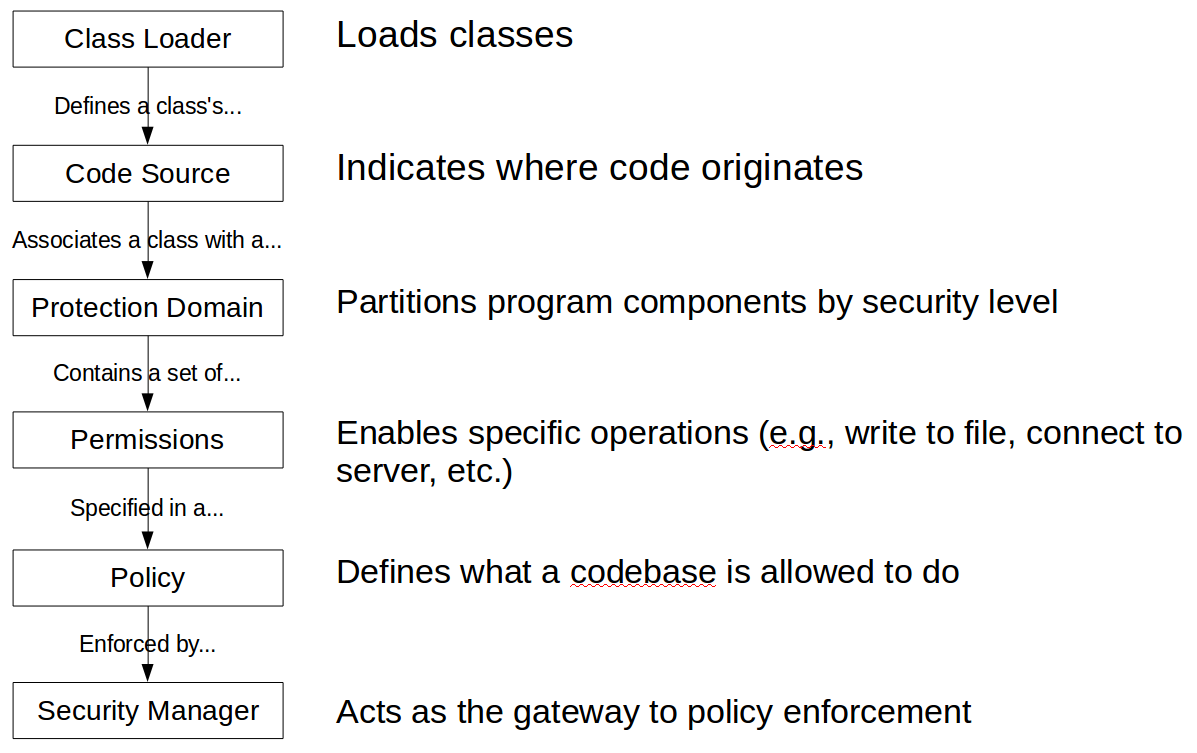
\includegraphics[scale=0.3]{sandbox_overview}

\caption{A summary of the components of the Java sandbox that are relevant
to understanding this work.}
\label{fig:Sandbox-high-level-summary}
\end{figure}


Defined policies will not be enforced unless the sandbox is activated.
The sandbox is activated by setting a security manager for the system.
This security manager acts as the gateway between the sandbox and
the rest of the application. Whenever a class attempts to execute
a method with security implications inside a sandbox, the protected
method queries the security manager to determine if the operation
should be allowed. For example, if an application attempts to write
to a file (e.g. \texttt{java.io.FileOutputStream}) inside a sandbox,
the class that performs the write will check with the security manager
to ensure that a write to that file is allowed. Missing checks are
a common source of Java vulnerabilities because protected code must
initiate the check. 

To perform a permission check, the security manager walks the call
stack to ensure each class in the current stack frame has the required
permission. However, privileged code can stop stack walking before
the entire frame has been walked by wrapping code inside a \texttt{doPrivileged}
call. This allows privileged code sections to perform actions with
security implications at the request of non-privileged code sections,
once the request has been properly verified. If the permission check
reaches a class in the stack frame that does not have the correct
permissions, the security manager will throw a \texttt{SecurityException}.
Stack-based access control is discussed in more detail in \cite{banerjee_stack-based_2005,besson_stack_2004,d._s._wallach_understanding_1998,erlingsson_irm_2000,fournet_stack_2002,pistoia_beyond_2007,zhao_type_2005}. 

Java is flexible about when in an application's execution the sandbox
is configured and enabled. The default case for web applets and applications
that use Java Web Start is to set a \textit{self-protecting} security
manager before loading the application from the network. The security
manager, and thus the sandbox, is self-protecting in the sense that
it does not allow the application to change sandbox settings. A security
manager can also be \textit{defenseless}, which is the exact opposite
of self-protecting. A defenseless manager does little to improve the
security of a constrained application or the host. However, we show
in Section \ref{sec:Study-results} that some benign applications
have found interesting uses for defenseless managers. 

Table \ref{tab:defenseless-permissions} summarizes the set of permissions
used to distinguish between self-protecting and defenseless security
managers. We consider any security manager that enforces a policy
that contains even one of the listed permissions to be defenseless.
A subset of the permissions in this list were identified in \cite{security_explorations_2012}. 

\begin{table*}
\caption{List of sandbox-defeating permissions. A security manager that enforces
a policy containing any of these permission is sufficient to result
in a defenseless sandbox.}
\label{tab:defenseless-permissions}


\centering{}%
\begin{tabular}{ll}
\toprule 
\textbf{Permission} & \textbf{Risk}\tabularnewline
\midrule
RuntimePermission(``createClassLoader'') & Load classes into any protection domain\tabularnewline
RuntimePermission(``accessClassInPackage.sun'') & Access powerful restricted-access internal classes\tabularnewline
RuntimePermission(``setSecurityManager'') & Change the application's current security manager\tabularnewline
ReflectPermission(``suppressAccessChecks'') & Allow access to all class fields and methods as if they are public\tabularnewline
FilePermission(``<\textcompwordmark{}<ALL FILES>\textcompwordmark{}>'',
``write, execute'') & Write to or execute any file\tabularnewline
SecurityPermission(``setPolicy'') & Modify the application's permissions at will\tabularnewline
SecurityPermission(``setProperty.package.access'') & Make privileged internal classes accessible\tabularnewline
\bottomrule
\end{tabular}
\end{table*}



\section{Exploiting Java Code} \label{sub:Java-Exploits}

This section provides an analysis of privilege escalation in the Java
security model and recent Java exploits. Between 2011 and 2013, drive-by
downloads that used Java applets as the vector were widely reported.
While the Java sandbox \textit{should} prevent malicious applets from
executing their payloads, exploits leveraged vulnerabilities in the
Java Runtime Environment (JRE) to set the security manager to \texttt{null}.
Setting the security manager to \texttt{null} disables the sandbox,
allowing previously constrained classes to perform any operation that
the JRE itself has the privileges to perform. Figure \ref{fig:A-typical-exploit-payload}
shows a typical payload class whose privileges have been elevated
by an exploit to allow it to disable the sandbox. This example payload
uses \texttt{doPrivileged} to allow the unprivileged exploit class
to execute the operations in the payload without causing a \texttt{SecurityException}.

\begin{figure}
\begin{centering}
\begin{lstlisting}[language=Java,basicstyle={\scriptsize}]
import java.lang.reflect.Method; 
import java.security.AccessController; 
import java.security.PrivilegedExceptionAction;   

public class Payload 
        implements PrivilegedExceptionAction {         
    public Payload() {
        try {
            AccessController.doPrivileged(this);
        } catch(Exception exception) { }     
    }

    public void run() {
        // Disable sandbox
        System.setSecurityManager(null);
    }

    public static void outSandbox() {
        // Do malicious operations
    }
}
\end{lstlisting}

\par\end{centering}

\caption{A typical sandbox-disabling Java exploit payload from http://pastebin.com/QWU1rqjf.}
\label{fig:A-typical-exploit-payload}
\end{figure}


Less than half of recent Java exploits use \textit{type confusion}
to bypass the sandbox. A type confusion vulnerability is exploited
by breaking type safety, allowing the attacker to craft an object
that can perform operations as if it is an instance of a class of
a different type. For example, attackers craft objects that either
(1) point to the \texttt{System} class or (2) act as if they have
the same type as a privileged class loader (see CVE-2012-0507 \cite{_vulnerability_2012_0507}).
In the first case the attack causes any operation performed on the
masqueraded class to happen on the real \texttt{System} class, allowing
the attacker to directly alter the field where the security manager
is stored. In the second case the malicious class can load the exploit's
payload with elevated privileges.

Another prominent class of Java exploits takes advantage of a \textit{confused
deputy} vulnerability \cite{hardy_confused_1988}, which is an example
of privilege escalation. In the case of a confused deputy, the exploit
often convinces a class with access to a vulnerable \textit{privileged
class} (i.e. a class with more privileges than the application's classes)
to return a reference to it. The returned privileged class often contains
a vulnerability such as a missing security check (e.g. where the class
should consult with the security manager before performing some operation,
but does not). In some cases, the privileged class may be directly
accessible to all Java applications, but this is quite rare and typically
the fault of a vulnerable third-party library. Providing all classes
with direct access to a privileged class is a violation of the \textit{access
control} principle that is part of the Java development culture.%
\footnote{\url{https://blogs.oracle.com/jrose/entry/the_isthmus_in_the_vm}%
} Once an exploit gains access to a vulnerable privileged class, that
class can be tricked into executing code that disables the sandbox
(see CVE-2012-4681 \cite{_vulnerability_2012_4681}).

For the most part, benign applications have no reason to directly
access privileged classes. The majority of the JRE's privileged classes
are internal implementations of features that applications can access
via less-privileged code paths. For example, many reflection operations
are implemented in the \texttt{sun.reflect} package, which has all
permissions. However, Java applications are supposed to use classes
in the \texttt{java.lang.reflect} package to use reflection and do
not have direct access to the \texttt{sun} classes given default JRE
configurations. Classes in the \texttt{java} package do not perform
privileged operations themselves, but do have permission to access
classes in the \texttt{sun} package.

A privileged class loader must be used to load a privileged class.
Thus, a class typically does not have direct access to a class that
has a vulnerability that can be exploited to bypass the sandbox unless
the former had its privileges reduced at some point in the application's
execution. This is implicit in the Java security model: If any class
could load more privileged classes and directly cause the execution
of privileged operations, the sandbox in its current form would serve
little purpose. In sections \ref{sec:Rules-for-Fortifying} and \ref{sec:Mitigations}
we discuss how we can leverage these distinctions to further fortify
the sandbox.

Many of the recent type confusion and privilege escalation vulnerabilities
would not have been introduced if the JRE were developed strictly
following ``The CERT Oracle Secure Coding Standard for Java'' \cite{long_cert_2011}.
For example, Svoboda \cite{svoboda_anatomy_blog_2013,svoboda_anatomy_2014}
pointed out that CVE-2012-0507 and CVE-2012-4681 were caused by violating
a total of six different secure coding rules and four guidelines. 

In the typical case, following just one or two of the broken rules
and guidelines would have prevented a serious exploit. For example,
CVE-2012-4681 resulted from two rule violations in a privileged Abstract
Window Toolkit (AWT) class in the \texttt{sun} package and two rule
violations and an ignored guideline in a JavaBean class. The bean
class was exploited to access the AWT class. The AWT class contained
a method that reflectively fetched any field in any class, made the
field public, and returned it. This is a violation of rule SEC05-J
because reflection is being used to increase the accessibility of
fields. It is also a violation of SEC00-J because the AWT class is
privileged and leaks sensitive information (the fields) across trust
boundaries. The AWT class should have followed all of the secure coding
guidelines, but its violation of SEC00-J is especially problematic---the
exploits use the leaked fields to disable the security manager. 

In the rest of this paper, we do not concern ourselves with the specifics
of particular exploits. We will now explore how benign applications interact with the sandbox to define ways of delineating them from exploits. 


\section{Introduction to the Security \\ Manager Study}\label{sec:Security-Manager-Study}

The nature of recent Java exploits caused us to ask the question: Do applications need access to any facility for disabling or weakening the sandbox? This study aims to answer this question and provide data in support of JVM enhancements to fortify the Java sandbox.
We focus our efforts on the security manager, as it is the means by
which applications interact with the sandbox. 

Any JVM enhancements that are to stop even zero-day exploits while maintaining backwards compatibility with benign applications must be designed with an understanding of which operations both exploitive
and benign applications perform on the security manager. Assuming
there is a difference between the set of operations performed by exploits
and those performed by benign applications, one can exclude the operations
on which exploits depend, that are not of use to benign applications. This strategy would help ensure the sandbox
continues to enforce its policy in a given execution without having
to deal with the wide diversity in the manifestations of vulnerabilities
within the JRE or the subtleties of their exploits. In this section
we describe the methodology for and limitations of an empirical study
that validated this strategy and answers our motivating question.


\subsection{Prior work}

Several recent studies have examined the use of security libraries
and discovered rampant library misuse, which caused severe vulnerabilities.
Georgiev et al. uncovered vulnerabilities in dozens of security critical
applications caused by SSL library protocol violations \cite{georgiev12most-dangerous}.
These applications misconfigured high-level libraries such that the
high-level libraries misused low-level SSL libraries which in turn
failed silently. Somorovsky et al. demonstrate vulnerabilities in
11 security frameworks such that Security Assertion Markup Language
(SAML) assertions are not checked properly when certain API mis-orderings
are triggered \cite{somorovsky12breaking}. Li et al. examined browser-based
password managers and found that many of their features relied on
an incorrect version of the same-origin policy, which could allow
attackers to steal user credentials \cite{li2014emperor}. As far
as we are aware no study has examined Java applications' use of the
sandbox. Li Gong, the main designer of the Java security architecture,
admitted in a ten year retrospective on Java Security that he didn't
know how or how extensively the ``fine grained access control mechanism''
(i.e. the Java sandbox) is used \cite{gong2009java}. We fill in that
gap. 


\subsection{Methodology}

As discussed in the previous sections, it is widely known within the
Java security community that current exploits that operate on the
security manager perform one operation: They disable it. To understand
the operations benign applications perform on the manager, we undertook
an empirical analysis consisting of static, dynamic, and manual inspections
of the open source Java application landscape. More precisely, we
answer the following research question: How do open source Java applications
interact with the security manager? To answer this question, our empirical
analysis aimed to validate four independent hypotheses. Each hypothesis
is paired with a mitigation that can be implemented if the hypothesis
is supported. The mitigations are given names that denote their relative
strengths when compared to each other. For example, a ``weak'' mitigation
stops a small number of in-scope exploits and is easily bypassed.
An ``ideal'' mitigation stops all in-scope exploits and can never
be bypassed. Our hypotheses and their accompanying mitigations follow: 

\textbf{Hypothesis 1:} \emph{Benign applications do not disable
the security manager.} If this hypothesis holds, exploits can be differentiated
from benign applications by any attempt to disable the current security
manager. This \textbf{weak mitigation} would be easy to implement,
but exploits that weaken the sandbox without disabling it would remain
a threat. For example, attackers could potentially bypass the mitigation
by modifying the enforced policy to allow the permissions they need
or they could replace the current manager with one that never throws
a \texttt{SecurityException}.

\textbf{Hypothesis 2:} \emph{Benign applications do not weaken the
security manager}. Validation of this hypothesis would enable
mitigations that prevent attackers from weakening or disabling the
sandbox. However, an implementation of this \textbf{moderate mitigation}
would require differentiating between changes which weaken the sandbox
and those that do not. Classifying changes in this manner autonomously is difficult
because it requires context specific information that a general mitigation
strategy may not have. For example, if a permission to write to a
file is replaced by a permission to write to a different file, is
the sandbox weakened, strengthened, or exactly as secure as it was
before?

\textbf{Hypothesis 3:} \emph{Benign applications do not change the
sandbox if a self-protecting security manager has been set}. If supported,
it is possible to implement a mitigation strategy that disallows any
change to a security manager that is enforcing a strict policy (as
defined in Section \ref{sec:Background}). To implement this \textbf{strong
mitigation}, a runtime monitor must determine if a security manager
is self-protecting at the time the manager is set. This can be easily
achieved. While this mitigation has the same outcome as the moderate
mitigation, it is significantly easier to implement soundly and it
is therefore more likely to be effective in practice. 

\textbf{Hypothesis 4:} \textit{Benign applications do not change a
set security manager.} If the study supports this hypothesis, any
attempted change to an already established security manager can be
considered malicious. The \textbf{ideal mitigation} could easily be
implemented in the JVM. 

Our empirical analysis used applications from the Qualitas Corpus
(QC) \cite{QualitasCorpus:APSEC:2010} and GitHub to form a dataset
of applications that use the security manager. To filter relevant
applications out of the 112 applications in QC, we performed a simple
\texttt{grep} of each application's source code to find instances
of the keyword \textit{SecurityManager}. When any instance of the
keyword was found, we included the application in our dataset. This
filtering reduced the set of applications to inspect from 112 to 29. 

We performed a similar process on GitHub while searching only Java files. The keyword \textit{System.setSecurityManager(} was added to remove false positives. To include applications that disable the manager we also searched for \textit{System.setSecurityManager(null)}. We picked the top seven applications from the results for each keyword, removed false positives, and ended up with an additional 17 applications that were not already in QC. We only looked at the latest commit.

With the dataset in hand, we created static and dynamic analysis tools
to assist in the manual inspection of each application. Our static
analysis tool is a FindBugs \cite{hovemeyer_finding_2004} plugin
that uses a dataflow analysis to determine where \texttt{System.setSecurityManager}()
is called, as well as the lines of code where its arguments were initialized.
We created a dynamic analysis tool using the Java Virtual Machine
Tool Interface (JVMTI) \cite{_jvmti}. JVMTI is designed to allow
tools to inspect the current state of Java applications and control
their execution; it is commonly used to create Java debugging and
profiling tools. Our dynamic analysis tool set a modification watch
on the \texttt{security} field of Java's \texttt{System} class. This
field holds the current security manager object for the application.
The watch prints out the class name, source file name, and line of
code where any change to the field took place. A special notice is
printed when the field is set to \texttt{null}. 

We split the dataset between two reviewers. The reviewers both analyzed
applications using the following steps:

\begin{enumerate}
\item Run grep on all Java source files in the application
to output every line containing the keyword \textsl{SecurityManager} and the 5 lines before and after it.
\item Reject any application where it is clear from the grep output that the keyword is used in ways that are unrelated to the security manager class.
\item Run the static analysis on retained applications. 
\item Manually inspect code specified in step 3's findings,
starting with the line where the manager was set and tracing the code
back to locations where potential security
managers were initialized. 
\item Manually inspect all of the lines returned in step 1, looking for how the application interacts with
the sandbox. 
\item Execute the application with the dynamic analysis using parameters
and actions steps 4 and 5 show affect the security
manager to verify conclusions from previous steps.
\item Summarize the operations performed
on the security manager with an emphasis on points that support or
reject each hypothesis.
\end{enumerate}

We undertook a pilot study where each reviewer
independently inspected the same six applications and compared their
results. This ensured reviewers understood the analysis steps and produced
consistent results.

\subsection{The Security Manager Dataset}\label{sec:Applications-Studied}

\begin{table}
\caption{Table of applications included in the security manager study.}
\label{Table:applications-studied}


\centering{}%
\begin{tabular}{lll}
\toprule 
Application Name & Description & Repo\tabularnewline
\midrule
(Apache) Ant & Java Project Builder & QC\tabularnewline
(Apache) Batik & SVG Image Toolkit & QC\tabularnewline
C-JDBC & DB Cluster Middleware & QC\tabularnewline
Compiere & Business Tools & QC\tabularnewline
(Apache) Derby & Relational Database & QC\tabularnewline
DrJava & IDE & QC\tabularnewline
Eclipse  & IDE & QC\tabularnewline
FreeMind & Mind-Mapping Tool & QC\tabularnewline
Galleon & Media Server & QC\tabularnewline
(Apache) Hadoop & Distrib. Comp. Frwk. & QC\tabularnewline
Hibernate & Obj.-Rel. Mapper & QC\tabularnewline
HyperSQL & SQL DB & QC\tabularnewline
JBoss & Application Middleware & QC\tabularnewline
JRuby & Ruby Interpreter & QC\tabularnewline
(Apache) Lucene & Search Software & QC\tabularnewline
(Apache) MyFaces & Server Software & QC\tabularnewline
NekoHTML & HTML Parser & QC\tabularnewline
Netbeans & IDE & QC\tabularnewline
OpenJMS & Messaging Service & QC\tabularnewline
Quartz  & Job Scheduler & QC\tabularnewline
QuickServer & TCP Server Frwk. & QC\tabularnewline
Spring Framework & Web Dev. Library & QC\tabularnewline
(Apache) Struts & Web Dev. Library & QC\tabularnewline
(Apache) Tapestry & Web Dev. Library & QC\tabularnewline
(Apache) Tomcat & Web Server & QC\tabularnewline
Vuze & File Sharing App. & QC\tabularnewline
Weka & Machine Learning Algs. & QC\tabularnewline
(Apache) Xalan & XML Trans. Library & QC\tabularnewline
(Apache) Xerces & XML Parsing Library & QC\tabularnewline
AspectJ & Java Extension & Github\tabularnewline
DemoPermissions & Spring Extension & Github\tabularnewline
driveddoc & Application Connector & Github\tabularnewline
FileManager- & FTP Server & Github \\ FtpHttpServer\tabularnewline
Gjman & Development Toolkit & Github\tabularnewline
IntelliJ IDEA & IDE & Github\tabularnewline
Jmin & Lightweight JDK & Github\tabularnewline
MCVersion-Control & Minecraft Utility & Github\tabularnewline
NGOMS & Business Tools & Github\tabularnewline
oxygen-libcore & Android Dev. Lib. & Github\tabularnewline
refact4j & Meta-model Prog. Frwk. & Github\tabularnewline
Security-Manager & Alt. Security Manager & Github\tabularnewline
Spring-Modules & Spring Extension & Github\tabularnewline
System Rules & JUnit Extension & Github\tabularnewline
TimeLag & Sound Application & Github\tabularnewline
TracEE & JavaEE Support Tool & Github\tabularnewline
Visor & Closure Library & Github\tabularnewline
\bottomrule
\end{tabular}
\end{table}


The Qualitas Corpus is a curated collection of open source Java applications
for use in reproducible software studies. We investigated sandbox
interactions in 29 applications from QC version 20130901.

\begin{table}
\caption{Classification of application interactions with the security manager.}
\label{tab:Classification-of-Application}

\centering{}%
\begin{tabular}{lrrr}
\toprule 
Type of Interaction & QC & GitHub & Total\tabularnewline
\midrule
1. Sets manager, nothing else & 6 & 1 & 7\tabularnewline
2. Changes set security manager & 5 & 3 & 8\tabularnewline
3. Support being sandboxed & 10 & 3 & 13\tabularnewline
4. Interactions only in unit tests & 3 & 5 & 8\tabularnewline
5. No interactions (false positive) & 5 & 5 & 10\tabularnewline
\bottomrule
\end{tabular}
\end{table}


While QC provides a strong starting point for the construction of
a dataset for this study, their inclusion criteria%
\footnote{http://qualitascorpus.com/docs/criteria.html%
} leads to the inclusion of large, popular applications and frameworks.
We diversified our dataset by turning to GitHub. Table \ref{Table:applications-studied}
lists all studied applications. Version numbers and Git commit hashes
are available in an online supplement.%
\footnote{http://goo.gl/dtcqTM%
}

\subsection{Limitations}\label{sub:Limitations-Study}

\subsubsection{Internal Validity}

Our results are dependent on accurately studying the source code of
applications and their comments. In most cases, security manager interactions
are easily understood, but there are a few particularly complex interactions
that may be misdiagnosed. Furthermore, we did not review all application
code, thus we may have taken a comment or some source code out of
context in larger applications. Finally, using two different reviewers
may lead to variations in the interpretations of some of the data. 

We mitigated these threats by using a checklist, FindBugs plugin, and JVMTI agent to
provide reviewers consistent processes for reviewing code
and validating their results. Furthermore,
we inspected entire source files that contained
security manager operations. We tested our tools and processes in a pilot study
to find and mitigate sources of inconsistencies.

\subsubsection{External Validity}

The study only includes open source applications. It is possible
that closed source applications interact with the security manager
in ways that we did not see in the open source community. However,
we inspected a few small applications with our aerospace collaborators.
We did not find any code that suggested this is the case. 

\subsubsection{Reliability}

While the majority of the study is easily replicable, GitHub search results are constantly
changing. Using GitHub to generate a new dataset using our method
would likely generate a different dataset. Furthermore, over the course of our security
manager study, two applications either became private repositories
or were removed from GitHub (FileManagerFtpHttpServer and Visor).

\section{Security Manager Study Results}\label{sec:Study-results}

We characterized the security manager interactions of the applications in our dataset by assigning each one of five types. The
types are summarized as follows: (1) applications that set a
security manager that does not get changed later in the application's
execution, (2) applications that change a set manager at some point
in the program's execution, (3) applications that interact with a
security manager in production code if one is set but do not modify the manager or its policy, (4) applications
that only interact with the manager in unit tests, and (5) false positives
that do not actually interact with the manager. Table \ref{tab:Classification-of-Application}
summarizes our dataset using these types.

Type 3, 4, and 5 applications will not be discussed further. The applications in these categories cannot violate any of our hypotheses because they do not attempt to alter a security manager or policy it enforces.

Type 1 and 2 applications provide the bulk of the material for the rest of this section because they set security managers to enforce policies and even change a manager or its policy after it has been set. Unlike Type 1 applications, Type 2 applications can violate our hypotheses. However, Type 1 applications are still of interest because they provide novel insights into how benign applications use the sandbox. At this point we stop distinguishing applications by their types to discuss application that use the sandbox for purposes that are not security related in Section \ref{sub:Non-security-uses-of}
and applications that use the sandbox for its intended security purposes in Section \ref{sub:Using-the-Security}.

\subsection{Evaluation of the Hypotheses}\label{sub:Evaluation-of-the-hypotheses}

We only require one counterexample to falsify a hypothesis from Section
\ref{sec:Security-Manager-Study}. This section summarizes how our
hypotheses held up against the results of this study.

\textbf{Hypothesis 1}: \emph{Benign applications do not disable
the security manager.} The investigation determined
that some benign applications do disable the security manager, which
turns off the sandbox. The applications that explicitly disabled the
manager typically were not using the sandbox for security purposes, but a few did to allow the user to update the security policy.

\textbf{Hypothesis 2}: \emph{Benign applications do not weaken the
security manager.} Multiple applications provided methods for the user to dynamically change the security policy or the manager in ways that can reduce the security of the sandbox.

\textbf{Hypothesis 3}: \emph{Benign applications do not change the
security manager if a self-protecting security manager has been set}.
This hypothesis was supported by both datasets.

\textbf{Hypothesis 4}: \emph{Benign applications do not change a
set security manager.} This hypothesis was falsified by multiple applications that changed the security manager.

In short, the strong mitigation is the only proposed mitigation that
can be implemented without breaking benign applications.

\subsection{Non-security uses of the Sandbox}\label{sub:Non-security-uses-of}

This section describes applications that provide novel insights into benign sandbox interactions unrelated to satisfy security
requirements. Most of these applications used the
sandbox to enforce architectural constraints when interacting with
other applications or forcibly disabled the sandbox to reduce development
complexity.

\subsubsection{Enforcing Architectural Constraints}

Java applications commonly call \texttt{System.exit()} when a non-recoverable
error condition occurs. This error handling strategy causes problems
when an application uses another application that implements this
strategy as a library. When the library application executes \texttt{System.exit()},
the calling application is closed as well because both applications
are running in the same JVM. In many cases, this is not the intended
outcome. 

To prevent this outcome without modifying the library application,
the calling application needs to enforce the architectural constraint
that libraries can not terminate the JVM. In practice, applications
enforce this constraint by setting a security manager
that prevents \texttt{System.exit()} calls. If a manager has already
been set, applications tend to save a copy of the current manager
before replacing it with one that prevents termination of the JVM,
but defer to the saved version for all security decisions that do
not have to do with enforcing this particular constraint. The original
security manager is often restored when the library application is
finished executing.

This case appears in Eclipse, which uses Ant as a library. When an
unrecoverable error condition occurs, Ant kills the JVM to terminate
execution of the build script currently running. However, Eclipse
should continue executing and report an error to the user when Ant
terminates with an error code. Figure \ref{fig:Eclipse-snippet} shows
how Eclipse sets a security manager to enforce this constraint right
before Ant is executed. After Ant closes and any error conditions
are handled, the original manager is restored.

\begin{figure}
\begin{lstlisting}[language=Java,numbers=left,basicstyle={\scriptsize},breaklines=true,firstnumber=691,xrightmargin={0.1cm},numbersep={-10pt}]
    System.setSecurityManager(new AntSecurityManager(originalSM, Thread.currentThread()));
    ...
\end{lstlisting}


\begin{lstlisting}[language=Java,numbers=left,basicstyle={\scriptsize},breaklines=true,firstnumber=703,xrightmargin={0.1cm},numbersep={-10pt}]
    getCurrentProject().executeTargets(targets); \\Note: Ant is executed on this line
    ...
\end{lstlisting}


\begin{lstlisting}[language=Java,numbers=left,basicstyle={\scriptsize},breaklines=true,firstnumber=721,xrightmargin={0.1cm},numbersep={-10pt}]
    finally {
    ...
\end{lstlisting}


\begin{lstlisting}[language=Java,numbers=left,basicstyle={\scriptsize},breaklines=true,firstnumber=725,xrightmargin={0.1cm},numbersep={-10pt}]
        if (System.getSecurityManager() instanceof AntSecurityManager) { 
            System.setSecurityManager(originalSM); 
        }
\end{lstlisting}


\protect\caption{Snippet of Eclipse code that uses a security manager to prevent Ant
from terminating the JVM when Ant encounters an unrecoverable error.}\label{fig:Eclipse-snippet}
\end{figure}

GJMan also enforces this constraint and contains a code comment referencing a
blog post that we believe is the origin of this solution.%
\footnote{http://www.jroller.com/ethdsy/entry/disabling\_system\_exit%
} 

In total, we found 3 applications that use a variation of this technique:
Eclipse, GJMan, and AspectJ. While this technique does enforce the
desired constraint, and appears to be the best solution available
in Java at the moment, it may cause problems when applications are
also using the sandbox for security purposes. The technique requires
the application to dynamically change the security manager. This operation
requires that the manager itself be defenseless or that the application
is very carefully written to prevent malicious code from changing
the manager or the policy it enforces. Defenseless security managers
are not capable of reliably enforcing a serious security policy.

\subsubsection{Reducing Web Application Development Complexity}\label{sub:Reducing-Web-Application-Complexity}

We found applications that were complicated by the Java security policies
for web applications (applets and applications launched via JWS). By default, Java executes such an application inside a restrictive
sandbox that severely limits the operations the application can perform,
excluding operations such as accessing local files, retrieving resources
from any third party server, or changing the security manager. 

Applications in our set that cannot run in a restrictive sandbox universally opted to run outside of the sandbox because the alternative is to painstakingly construct the application to run reasonably without required privileges (e.g. by detecting the sandbox and disabling privileged operations). To avoid executing the applet in a restrictive
sandbox, a developer must get the application digitally signed
by a recognized certificate authority then specify that the application should
run outside of the sandbox. We found that applications using this method attempted
to set the security manager to \texttt{null} at the beginning of the
application, causing a restrictive sandbox to catch the security violation and
terminate the application.

We found two applications that use the second option: Eclipse and
Timelag. The rationale for disabling the manager in Eclipse is explained in a code comment that reads, "The launcher to start eclipse using webstart. To use this launcher, the client must accept to give all security permissions." Timelag performs the same operation in the file JTimelag.java but does not contain any comments, thus we can only infer the motivation behind turning off the sandbox.

\subsection{Using the Security Manager for Security Purposes}\label{sub:Using-the-Security}

This section describes applications that provide novel insights into benign sandbox interactions related to improving the security
posture of the application. Several of these applications clearly violate hypotheses 1, 2, and 4: Batik, Eclipse, and Spring-modules provide
methods that allow the user to set and change an existing manager,
and Ant, Freemind, and Netbeans explicitly set then change the manager.

\begin{figure}
\begin{lstlisting}[language=Java,numbers=left,basicstyle={\scriptsize},breaklines=true,firstnumber=156,xrightmargin={0.1cm},numbersep={-10pt}]
    public void enforceSecurity(boolean enforce){ 
    SecurityManager sm = System.getSecurityManager();

    if (sm != null && sm != lastSecurityManagerInstalled){
        ...
\end{lstlisting}


\begin{lstlisting}[language=Java,numbers=left,basicstyle={\scriptsize},breaklines=true,firstnumber=163,xrightmargin={0.1cm},numbersep={-10pt}]
        throw new SecurityException
            (Messages.getString(EXCEPTION_ALIEN_SECURITY_MANAGER));   
    }                  
    if (enforce) { 
        ...
\end{lstlisting}


\begin{lstlisting}[language=Java,numbers=left,basicstyle={\scriptsize},breaklines=true,firstnumber=173,xrightmargin={0.1cm},numbersep={-10pt}]
        installSecurityManager();         
    } else {             
        if (sm != null) {                 
           System.setSecurityManager(null);
           lastSecurityManagerInstalled = null;             
           ...
\end{lstlisting}


\protect\caption{Security manager interactions in Batik.}\label{fig:Batik-snippet}
\end{figure}


Figure \ref{fig:Batik-snippet} shows an interesting case from Batik
copied from \texttt{ApplicationSecurityEnforcer.java}. This method
allows users to optionally constrain the execution of an an application
that uses the Batik SVG Toolkit. It takes a parameter that acts as
a switch to turn the sandbox on or off. The download page on the Batik
website shows several examples of how to use the library. Two set
a security manager at start up: the squiggle browser demo and the
rasterizer demo. While the squiggle browser demo sets a manager and
never changes it, the rasterizer demo calls \texttt{enforceSecurity}
with a true argument the first time and a false argument the second
time, which enables then disables the sandbox. While this was an interesting
occurrence, there seems to be no valid reason to disable the sandbox
in this case other than to show off the capability to do so.

Ant, Freemind, and Netbeans explicitly set and then change the manager
during runtime. Ant allows the users to create build scripts that
execute Java classes during a build under a user specified
permissions set. Figure \ref{fig:Ant Permissions Example}
shows the first example of a permission set from the Ant Permissions website.%
\footnote{https://ant.apache.org/manual/Types/permissions.html%
} The contents of the \texttt{grant} element provide the application
all permissions, but the contents of the \texttt{revoke} element restrict
the application from using all property permissions. Due the use a
defenseless security manager, malicious code can easily disable the sandbox and perform all actions
including those requiring \texttt{PropertyPermissions}.

\begin{figure}
\begin{lstlisting}[language=XML,basicstyle={\scriptsize}]
<permissions>   
  <grant class="java.security.AllPermission"/>   
  <revoke class="java.util.PropertyPermission"/> 
</permissions>
\end{lstlisting}

\caption{Example Ant build script element to grant all but one permission.
This specific permission set leads to a defenseless security manager.}
\label{fig:Ant Permissions Example}
\end{figure}

When Ant is about to execute an external, constrained class, it saves the current security manager and replaces it with a custom manager. This operation assumes the current manager is defenseless. The custom manager is not defenseless given a self-protecting permission set, but contains a private switch to make the manager defenseless for the purposes of restoring the original manager. With this implementation, Ant catches applications that perform actions
restricted by the user while typically protecting sandbox settings. However, it is not clear this implementation
is free of vulnerabilities.

Netbeans similarly sets a security manager around a separate application.
Both of these cases require a defenseless security manager, otherwise
the application would not be able to change the current security manager.
A better implementation would use a custom class
loader to load the untrusted classes into a constrained protection
domain. This approach would align with the intended usage of the sandbox.
Additionally, it would be more clearly correct and trustworthy while
allowing Ant and Netbeans to run inside of a self-protecting sandbox.

Freemind 0.9.0 tried to solve a similar problem but ended up illustrating
the dangers of a defenseless manager. Freemind is a mind mapping tool
that allows users to execute Groovy scripts on an opened map. The
scripts are written by the creator of the mind map. Groovy is a scripting
language that is built on top of the JRE: A Java application that
executes a script typically allows the script to execute in the same
JVM as the application itself. As a result, a mind map could potentially
be crafted to exploit a user that opens the map and runs its scripts.

\begin{figure}
\begin{lstlisting}[numbers=left,basicstyle={\scriptsize},breaklines=true,firstnumber=30,xrightmargin={0.1cm},numbersep={-10pt}]
  /**  
   * By default, everything is allowed.  
   * But you can install a different security controller once,  
   * until you install it again. Thus, the code executed in   
   * between is securely controlled by that different security manager.  
   * Moreover, only by double registering the manager is removed. So, no   
   * malicious code can remove the active security manager.  
   *   
   * @author foltin  
   *  
   */
   public void setFinalSecurityManager(SecurityManager pFinalSecurityManager) {
	 if(pFinalSecurityManager == mFinalSecurityManager){
       mFinalSecurityManager = null;
	   return;
      } 		
      if(mFinalSecurityManager != null) {
      throw new SecurityException("There is a SecurityManager installed already."); 		
      } 		
      mFinalSecurityManager = pFinalSecurityManager;
    }	
\end{lstlisting}


\caption{Initialization of the field in Freemind's custom security manager
that stores the proxy security manager.}
\label{fig:Freemind-Security-Manager}
\end{figure}

Freemind attempted to implement an architecture that would allow the
sandbox to enforce a stricter policy on the Groovy scripts than on
the rest of Freemind. Their design centers around the use of a custom
security manager that is set as the system manager in the usual manner.
This custom manager contains a field, \texttt{mFinalSecurityManager},
that specifies the proxy manager to be used during the execution of
scripts. In this design, all checks to the security manager are ultimately
deferred to the proxy manager set in this field. When
this field is set to \texttt{null}, the sandbox is effectively disabled
even though the system's manager is still set to the custom manager.

Figure \ref{fig:Freemind-Security-Manager} shows how Freemind sets
the proxy security manager field in the file \texttt{FreemindSecurityManager.java}.
Once a manager is set, if \texttt{setFinalSecurityManager} is called
again with a different security manager, a \texttt{SecurityException}
is thrown, but calling the method with a reference to the set manager disables the sandbox. The comment implies this specific sequence
of operations was implemented to prevent malicious applications from
changing the settings of the sandbox.

The Freemind code responsible for initiating the execution of the
Groovy scripts sets a proxy security manager that does not allow unsigned
scripts to create network sockets, access the file-system, or execute
programs on the machine. The manager explicitly allows all other permissions by overriding permission check methods with implementations that do nothing. As a result, a malicious script can turn off the sandbox at any point.

We demonstrated that the custom security manager is easily removed
using reflection to show that the problem is more complex than simply
fixing permission checks related to setting the security manager. Figure \ref{fig:Example-Exploit-for-Freemind}
shows a Groovy exploit to turn off the manager. The script gets a reference to the system's manager
and its class. The class has the same type as the custom security
manager, thus the exploit gets a reference to the proxy manager field.
The field is made public to allow the exploit to reflectively \texttt{null}
it, disabling the sandbox to allow ``forbidden'' operations.

We sent a notice to the Freemind developers in August of 2014 to provide
them with our example exploit and to offer our advice in achieving
their desired outcome. 

\begin{figure}
\begin{lstlisting}[language=Java,basicstyle={\scriptsize},breaklines=true]
def sm = System.getSecurityManager() 
def sm_class = sm.getClass() 
def final_sm = sm_class.getDeclaredField("mFinalSecurityManager")
final_sm.setAccessible(true) 
final_sm.set(sm, null)
new File("hacked.txt").withWriter { out -> out.writeLine("HACKED!") }
\end{lstlisting}


\caption{Example exploit that breaks out of the scripting sandbox in Freemind
to execute arbitrary code.}
\label{fig:Example-Exploit-for-Freemind}
\end{figure}

\section{Rules for Fortifying the Sandbox}\label{sec:Rules-for-Fortifying}

Given the results of our investigation in Section \ref{sec:Security-Manager-Study}
and the discussion in Section \ref{sub:Java-Exploits}, we can fortify
the sandbox for applications that set a\emph{ self-protecting} security
manager. In this section, we define two rules to stop Java exploits
from disabling the manager. These rules are backwards-compatible with
benign applications: the Privilege Escalation rule and the Security
Manager rule. 

\subsection{Privilege Escalation Rule}

The \textit{Privilege Escalation rule} ensures that, if a self-protecting
security manager is set for the application, a class may not directly
load a more privileged class. This rule is violated when the protection
domain of a loaded class implies a permission that is not implied
in the protection domain that loaded it. About half of recent exploits
break this rule to elevate the privileges of their payload class.

If all classes in the Java Virtual Machine (JVM) instance were loaded
at the start of an application, this rule would never be broken. However,
the JVM loads certain classes on demand, and some of the JVM classes
have the full privileges. Classes in
packages that are listed in the \texttt{package.access} property of
\texttt{java.security.Security} are not subject to this rule because they are intended to be
loaded when accessed by a trusted proxy class. 

\subsection{Security Manager Rule}

The \textit{Security Manager rule} states that the manager cannot
be changed if a \emph{self-protecting} security manager has been set
by the application. This rule is violated when code causes a change
in the sandbox's configuration, the goal of many exploits. This rule
is an implementation of the strong mitigation.

\section{Validating the Rules}\label{sec:Mitigations}

In Section \ref{sec:Security-Manager-Study}, we discussed four hypotheses about security manager usage in benign applications, each
of which, if validated, leads to a distinct mitigation. In Section
\ref{sec:Study-results}, we gave empirical evidence in support of
Hypothesis 3 and rejected all of the others. Along the way, we learned
practical lessons about how applications use the Java sandbox that
are useful to exploit mitigation implementers. 

In this section, we evaluate the protection merits and backwards compatibility of the rules presented in Section \ref{sec:Rules-for-Fortifying} through an implementation of runtime monitors that enforce them. This evaluation was done in collaboration
with a large aerospace company.

Section \ref{sub:Implementation-Using-JVMTI} discusses how we implemented
our runtime monitors using JVMTI. Section \ref{sub:Effectiveness-at-Fortifying}
explains the methodology behind and results of an experiment we conducted
to determine how effective the rules are at stopping existing exploits without breaking benign applications. Finally, Section
\ref{sub:Related-Work-Mitigation} covers prior work related to Java exploit mitigations.

\subsection{Implementation Using JVMTI}\label{sub:Implementation-Using-JVMTI}

JVMTI is a native interface used to create
analysis tools such as profilers, debuggers, monitors, and thread
analyzers. Tools that use JVMTI are called agents, and are attached
to a running Java application at a configuration-specific point in
the application's lifecycle. The interface allows an agent to set
capabilities, enabling the tool to intercept events such as class
or thread creation, field access or modification, breakpoints, etc.

Our agent \footnote{Our agent is open source. An anonymized version
of the tool can be found at http://goo.gl/In6Di0} must intercept three events to enforce the Privilege Escalation
and Security Manager rules: \texttt{ClassPrepare}, \texttt{FieldAccess},
and \texttt{FieldModification}. Enforcement of these rules is discussed
in detail in subsections \ref{sub:Enforcing-the-Privilege} and \ref{sub:Enforcing-the-SecurityManager}.

The field events require JVMTI to turn off the JIT, which slows down program execution enough that our monitors are not suitable for adoption on their own. JVMTI implementations can avoid this limitation, but avoidance would likely increase implementation complexity beyond what is reasonable for a diagnostic interface. We are currently in communication with the OpenJDK developers on their security-dev mailing list regarding enforcement of our rules in the JVM itself to avoid overhead issues.\footnote{REVIEWERS: This discussion will be referenced in the final version of the paper. At this time, the OpenJDK developers are very receptive to the idea, were already considering implementing something similar to our SecurityManager rule, and have stated the lessons from the empirical study we shared with in an early manuscript of this paper are valuable to their efforts.}

\subsubsection{Enforcing the Privilege Escalation Rule}\label{sub:Enforcing-the-Privilege}

The Privilege Escalation rule is enforced by ensuring that classes
can only load or cause the loading of more privileged classes in restricted-access
packages after a self-protecting security manager has been set. \textit{Restricted-access
packages} are packages that are public but not intended to be directly
used by typical Java applications; they are meant for internal JRE
use only. These packages are listed in the \texttt{package.access}
property in the \texttt{java.security.Security} class. There are two
ways to unsafely and directly access packages listed in this property:
(1) exploit a vulnerability in a class that can access them or (2)
allow access via the \texttt{accessClassInPackage} permission.

Applications use JRE classes which call restricted access package
classes. Thus, we must allow JRE to load restricted-access packages
at runtime. For example, many of the classes in the \texttt{java.lang.reflect}
package are backed by classes in the \texttt{sun} package, which is
a restricted-access package containing the internal implementations
for many Java features. However, enforcing the Privilege Escalation
rule prevents exploits from elevating the privileges of their payloads
because the payloads can not be in restricted-access packages with
default JRE configurations. 

To enforce the Privilege Escalation rule, our agent registers for
the \texttt{ClassPrepare} event, which allows the agent to inspect
a class after it is fully loaded but just before any of its code is
executed. Assuming the loaded class is not in a restricted-access
package, the agent inspects the stack frame to determine which class
caused the new class to be loaded. The agent must get the protection
domains for both classes. This can not be done from the agent using
the JNI because the required Java calls%
\footnote{\texttt{Class.getProtectionDomain()}%
} will be performed with the same permissions as the executing Java
application. Most applications where this operation is relevant (i.e.
those that have a self-protecting manager) do not have the necessary
permission%
\footnote{\texttt{RuntimePermission("getProtectionDomain")}%
} to get a protection domain because the permission would allow a malicious
class to probe the policy to determine which, if any, malicious operations
it can perform. Because JVMTI agents are loaded into the JRE as a
shared library, we instead load libjvm.so (jvm.dll on Microsoft Windows)
to call JVM functions without security checks. Our agent leverages
this ability to call the \texttt{GetProtectionDomain} JVM function
to get the protection domains. 

With both protection domains, the current agent implementation simply
checks to see whether the loaded class's protection domain has all
permissions while the class that caused the loading does not. If the
latter is true, the Privilege Escalation rule has been violated. This
specific check was used because it is fast, simple, and all privileged
classes allow all permissions under known circumstances. It would
be easy to update this check to instead ensure that every permission
in the loaded class's protection domain is also implied by the other
protection domain to handle other cases.

\subsubsection{Enforcing the SecurityManager Rule}\label{sub:Enforcing-the-SecurityManager}

The SecurityManager rule is enforced by monitoring every read from
and write to the \texttt{security} field of the \texttt{System} class:
This field stores the security manager that is used by protected code.
The agent implements the read and write monitors by respectively registering
\texttt{FieldAccess and FieldModification} events for the field. Typically
the field is accessed via \texttt{System.getSecurityManager()}
and modified using \texttt{System.setSecurityManager()}, but we must
monitor the field instead of instrumenting these methods to detect
type confusion attacks. 

The agent stores a shadow copy of the application's most recent security
manager to have a trusted copy of the manager that can be used to
check for rule violations. In a typical deployment, the agent is loaded
by a JVM before the hosted Java application's code has begun executing.
Even in the typical case, when a security manager is set on the command
line that runs the application, the initial security manager would
not be caught by the modification event because the write happens
before the agent is loaded. To solve this problem, the shadow copy
is first initialized by calling \texttt{System.getSecurityManager()}
when a JVM loads the agent. After this point, the shadow copy is only
updated by the modification event, which receives the new manager
as a parameter from JVMTI whenever the event is triggered.

Modification events are used to detect any change to a self-protecting
security manager. When the field is written, the agent checks the
shadow copy of the manager. Assuming the shadow copy is \texttt{null},
the agent knows the manager is being set for the first time and checks
to see if the new manager is self-protecting. If the manager is self-protecting
the agent simply updates the shadow copy. Otherwise the agent stops monitoring the application because the rule does not apply in the presence of a defenseless manager.

Access events are used to detect type confusion attacks against the
manager. The modification event we register will not be triggered
when the manager is changed due to a type confusion attack. When a
type confusion attack is used to masquerade a malicious class as the
\texttt{System} class, the malicious copy will have different internal
JVM identifiers for the class itself and its methods. Even given these
differences, updating a field in one version of the class updates
the value the JVM stores for the field in both classes because\texttt{
System} is static and both classes appear to have the same type. The
modification and access events are registered for specific field and
class identifiers, thus the events are not triggered for operations
on the malicious version. We leverage the mismatch this causes between
the set security manager and our shadow copy by checking to see if
the manager that is read in the access event has the same internal
JVM reference as our shadow copy. When the two references do not match,
the manager has been changed by a malicious class masquerading as
\texttt{System}. Type confusion attacks may also be used to masquerade
a class as a privileged class loader to elevate the privileges of
a payload class that disables the manager; this scenario is detected
by the modification event.


\subsection{Effectiveness at Fortifying the Sandbox}\label{sub:Effectiveness-at-Fortifying}

%%Need to integrate backwards compatibility experiment here

We performed an experiment to evaluate how effective our rules are
at blocking exploits that disable the sandbox. In our experiment,
we ran Java 7 exploits for the browser from Metasploit 4.10.0 on 64-bit
Windows 7 against the initial release of version 7 of the JRE. This
version of Metasploit contains twelve applets that are intended to
exploit JRE 7 or earlier, but two did not successfully run due to
Java exceptions we did not debug. Metasploit contains many Java exploits
outside of the subset we used, but the excluded exploits either only
work against long obsolete versions of the JRE or are not well positioned
to be used in drive-by downloads. 

We ran the ten exploits in our set under the following conditions:
(1) without the agent, (2) with the agent but only enforcing the Privilege
Escalation rule, and (3) while enforcing both rules. We ran these
conditions to respectively: (1) establish that the exploits succeed
against our JRE, (2) test how effective the Privilege Escalation rule
is without the security manager rule, and (3) evaluate how effective
the agent is in the strictest configuration. Overall, all
ten of the exploits succeed against our JRE without the agent. Four
were stopped by the Privilege Escalation rule. All ten were stopped
when both rules were enforced. The exploits that were not stopped
by the Privilege Escalation rule were either type confusion exploits
or exploits that did not need to elevate the privileges of the payload
class. The payload class does not need elevated privileges when it
can directly access a privileged class to exploit. Table \ref{tab:Exploit-experiment-summary}
summarizes our results using the specific CVEs each exploit targeted.

\begin{table}
\protect\caption{Effectiveness test results.}\label{tab:Exploit-experiment-summary}


\centering{}%
\begin{tabular}{l>{\raggedright}p{3cm}l}
\toprule 
\textbf{CVE-ID} & \textbf{Privilege Escalation Monitor} & \textbf{Both Monitors}\tabularnewline
\midrule
2011-3544 & Attack Succeeded  & Attack Blocked\tabularnewline
2012-0507 & Attack Blocked & Attack Blocked\tabularnewline
2012-4681 & Attack Succeeded  & Attack Blocked\tabularnewline
2012-5076 & Attack Succeeded  & Attack Blocked\tabularnewline
2013-0422 & Attack Blocked & Attack Blocked\tabularnewline
2013-0431 & Attack Blocked & Attack Blocked\tabularnewline
2013-1488 & Attack Succeeded  & Attack Blocked\tabularnewline
2013-2423 & Attack Succeeded  & Attack Blocked\tabularnewline
2013-2460 & Attack Blocked & Attack Blocked\tabularnewline
2013-2465 & Attack Succeeded  & Attack Blocked\tabularnewline
\bottomrule
\end{tabular}
\end{table}

\subsection{Related Work}\label{sub:Related-Work-Mitigation}

Our rules increase the security of the sandbox
by effectively removing unnecessary features. Prior work has taken a different
approach, instead focusing on re-implementing the Java sandbox or
adding to the sandbox to increase security. Cappos et al. created
a new sandbox structure. They implemented a security isolated kernel
to separate sandboxed applications from the main system \cite{cappos_retaining_2010}.
They validated this structure by translating past Java CVEs into exploits
for the new kernel. Provos et al. describe a method of separating
privileges to reduce privilege escalation \cite{Provos-PrivilegeEscalation}.
Their approach is partially implemented in the Java security model.
Li and Srisa-an extended the Java sandbox by providing extra protection
for JNI calls \cite{li_quarantine:_2011}. Their implementation, Quarantine,
separates JNI accessible objects to a heap which contains extra protection
mechanisms. The performance of their mechanism is also measured using
DaCapo. Siefers et al. created a tool, Robusta, which separates JNI
code into another sandbox \cite{siefers_robusta:_2010}%
\begin{comment}
Cite TISSEC journal version of Robusta paper
\end{comment}
. Sun and Tan extend the Robusta technique to be JVM independent \cite{sun_jvm-portable_2012}. 

Java applets are the most common ways to transmit Java exploits. Detectors
have been created to identify drive-by downloads in JavaScript \cite{cova_detection_2010},
and in Adobe Flash \cite{ford_analyzing_2009}. Helmer et al. used
machine learning to identify malicious applets \cite{helmer_anomalous_2001}.
Their approach monitored system call traces to identify malicious
behavior after execution. However, this approach is entirely reactive.
Our approach terminates exploits when they attempt to break out of
the sandbox, before the exploit performs its payload. Schlumberger
et al. used machine learning and static analysis to identify common
exploit features in malicious applets \cite{schlumberger_jarhead_2012}.
Blasing et al. used static analysis and dynamic analysis of sandboxed
executions to detect malicious Android applications \cite{Blasing-AndriodSandbox}.
Unlike these automated approaches, our rules shows that unique
mitigation strategies can be created with a better understanding of
how applications interact with the sandbox. 

\subsection{Limitations}

Neither of these rules will stop all Java exploits. While the rules
catch all of the exploits in our set, some Java vulnerabilities can
be exploited to cause significant damage without disabling the security
manager. For example, our rules will not detect type confusion exploits
that mimic privileged classes to perform their operations directly.
However, our rules substantially improve Java sandbox security, and
future work will be able to build upon these results to create mitigation
techniques for additional types of exploits.

\section{Conclusion}

Our study of Java sandbox usage in open-source applications found
that the majority of studied applications do not change the security
manager. Some of the remaining applications use the security manager
only for non-security purposes. The final set of applications use
the sandbox for security and either initialize a self-protecting security
manager and never modify it or set a defenseless manager and modify
it at run time. 

These findings, in combination with our analysis of recent Java exploits,
enabled us to define two rules which together successfully
defeated Metasploit's applet exploits without breaking backward compatibility with benign applications when enforced by an experimental JVMTI agent. Some of the studied applications
used the security manager to prevent third party components from calling
\texttt{System.exit()}. More generally, frameworks often need to enforce
constraints on plugins (e.g. to ensure non-interference). This suggests
that Java should provide a simpler, alternative mechanism for constraining
access to global resources. This is supported by our findings that
show developers attempting to make non-trivial use of the sandbox
often do so incorrectly. One intriguing possibility is to allow programmers
to strengthen the policy temporarily (e.g. by adding a permission). 

We indirectly observed many developers struggling to understand and
use the security manager for any purpose. This is perhaps why there
were only 46 applications in our sample. Some developers seemed to
misunderstand the interaction between policy files and the security
manager that enforces the policy. Other developers appear confused
about how permissions work. In particular, they do not realize that
restricting just one permission but allowing all others enables a
\emph{defenseless} sandbox. Our concerns are shared by the IntelliJ developers, who included static analysis checks to warn developers that a security expert should check their interactions with the security manager.\footnote{http://www.jetbrains.com/idea/documentation/inspections.jsp%
} In general, sandbox-defeating permissions
should be packaged and segregated to prevent accidental creation of
defenseless sandboxes. More generally, some developers appear to believe
the sandbox functions as a blacklist when, in reality, it is a whitelist.
These observations suggest that more resources---tool support, improved
documentation, or better error messages---should be dedicated to helping
developers correctly use the sandbox. 

\bibliographystyle{ieeetr}
\bibliography{references}

\end{document}
